\section{Specific Cases of Minimal Surfaces}
Having defined a minimal surface using Differential Geometry, we now ask what minimal surfaces actually exist and how do we find them? We will start by setting up a partial differential equation known as the minimal surface equation. However it will quickly become apparent that a general solution of this equation is not possible, we will therefore impose various geometric and algebraic constraints which will then allow us to solve for different classes of minimal surfaces.

\subsection{The Minimal Surface Equation}
Locally all surfaces can be defined by a Monge parametrisation  $z= f(x,y)$ so

\begin{displaymath}
\mathbf x(u,v) = (x, y, f(x,y))
\end{displaymath}

Calculating the first and second fundamental forms gives:

\begin{displaymath}
E = 1 + f_x^2 \ \ F = f_xf_y \ \ G = 1+f_y^2
\end{displaymath}

\begin{displaymath}
L = \frac{f_{xx}}{\sqrt{1+f_x^2+f_y^2}} \ \ M = \frac{f_{xy}}{\sqrt{1+f_x^2+f_y^2}} \ \ N = \frac{f_{yy}}{\sqrt{1+f_x^2+f_y^2}}
\end{displaymath}

Subbing these into our equation for Mean Curvature (Equation \ref{equ:H}) and equating to zero gives:
\begin{equation}
\framebox{$f_{xx}(1+f_y^2)-2f_{xy}f_xf_y+f_{yy}(1+f_x^2)=0$}
\label{equ:MinimalSurfaceEquation}
\end{equation}
Unfortunately in general this is not solvable by simple means. If we look for a surface defined globally we discover that the only such minimal surface is the plane, this is known as Bernstein's Theorem.
\begin{theorem}[Bernstein]
If a minimal surface $M: \, z=f(u,v)$ is defined on the whole xy-plane, then M is a plane.
\end{theorem}

However locally there are many such minimal surfaces, one of the most famous of these is \emph{Scherk's First Surface}.

\subsection{Scherk's First Surface}
We've already derived the minimal surface equation and said that it is not solvable by simple means however; we will apply an algebraic condition which will make the equation solvable.

We will look for surfaces with $f(x,y) = g(x) + h(y)$. Such surfaces are known as translation surfaces but we are interested in them because it allows us to separate variables leaving us with two ordinary differential equations which we can solve.

Letting $\mathbf x(x,y) = (x, y, g(x) + h(y))$ and following the same procedure as for the \emph{Minimal Surface Equation} (or in fact subbing $f(x,y) = g(x) + h(y)$ directly into equation \ref{equ:MinimalSurfaceEquation}). This gives us

\begin{equation}
g_{xx}(x)(1+h_y^2(y))+h_{yy}(y)(1+g_x^2(x)) = 0 
\label{equ:ScherkMinSurf}
\end{equation}

Rearranging gives

\begin{displaymath}
-\frac{1+g_x^2(x)}{g_{xx}(x)} = \frac{1+h_y^2(y)}{h_{yy}(y)}
\end{displaymath}

Now note that the LHS is a function of only x and the RHS is a function of only y. Varying one of these and holding the other fixed therefore cannot change anything, e.g. both sides are equal to the same constant.

\begin{displaymath}
-\frac{1+g_x^2(x)}{g_{xx}(x)} = c = \frac{1+h_y^2(y)}{h_{yy}(y)}
\end{displaymath}

This gives us two ordinary differential equations which we can then solve to find $g(x)$ and $h(y)$.

\begin{eqnarray}
\label{equ:Scherk_g}
1+g_x^2(x) &=& - cg_{xx}(x) \\
\label{equ:Scherk_h}
1+h_y^2(y) &=& ch_{yy}(y)
\end{eqnarray}

Both of these equation solve in exactly the same way (obviously noting the minus sign in \ref{equ:Scherk_g}). We will therefore just solve \ref{equ:Scherk_g} and state the result for \ref{equ:Scherk_h}.

Equation \ref{equ:Scherk_g} has no dependence on g(x), so we can set $\phi = g_x(x)$ which gives us

\begin{displaymath}
1+\phi^2 = -c\phi_x
\end{displaymath}

We can now separate and integrate:
\begin{displaymath}
\int\frac{-c}{1+\phi^2}d\phi = \int dx
\end{displaymath}

Letting $\phi = \tan \theta$ giving $\frac{d\phi}{d\theta} = \sec^2\theta$ and subbing in:

\begin{eqnarray}
\nonumber
\int\frac{-c}{1+\tan^2\theta}\sec^2\theta d\theta &=& \int dx \\
\nonumber
\Leftrightarrow \int\frac{-c}{\sec^2\theta}\sec^2\theta d\theta &=& \int dx \\
\nonumber
\Leftrightarrow \int\frac{-c}{\sec^2\theta}\sec^2\theta d\theta &=& \int dx \\
\nonumber
\Leftrightarrow -c\int d\theta &=& \int dx \\
\nonumber
\Leftrightarrow -c\theta &=& x \mbox{\ \ \ \ supressing constant of integration} \\
\nonumber
\Leftrightarrow -c \arctan \phi &=& x \\
\nonumber
\therefore \phi &=& -\tan\left(\frac{x}{c}\right)
\end{eqnarray}

Now re-writing in terms of g(x) gives:

\begin{displaymath}
g_x(x) = -\tan\left(\frac{x}{c}\right)
\end{displaymath}

Integrating this up gives

\begin{displaymath}
g(x) = c \ln\left((\cos \left(\frac{x}{c}\right)\right)
\end{displaymath}

Following this method exactly but taking the change of sign into account for equation \ref{equ:Scherk_h} gives

\begin{displaymath}
h(y) = -c \ln\left(\cos \left(\frac{y}{c}\right)\right)
\end{displaymath}
 
Putting these back together we get our $f(x,y)$.

\begin{eqnarray}
\nonumber
f(x,y) &=& g(x) + h(y) \\
\nonumber
&=& c \ln(\cos \left(\frac{x}{c}\right))-c \ln(\cos \left(\frac{y}{c}\right)) \\
\label{equ:Scherk_f}
&=& c \ln\left(\frac{cos(x/c)}{cos(y/c)}\right)
\end{eqnarray}

The surface $z=f(x,y)$ is known as \emph{Scherk's (first) minimal surface}. Since the logarithm function is only defined for positive values, Scherk's surface is only defined for $\frac{cos(x/c)}{cos(y/c)} > 0$. Therefore, for example letting $c=1$, Scherk's surface forms a chess board pattern with the surface defined on squares with vertices at points $\left(\frac{\pi}{2}+m\pi,\frac{\pi}{2}+n\pi\right)$, where m and n are integers. This can be seen in Figure \ref{fig:scherk}.

\begin{figure}[htbp]
	\centering
       \includegraphics[width=8cm]{Images/Scherk.eps}
   \caption{Scherk's First Minimal Surface}
   \label{fig:scherk}
\end{figure} 

\subsection{Surfaces of Revolution}
We have just seen what happens when we impose an algebraic condition on the minimal surface equation; however we can also impose geometric conditions in order to find minimal surfaces. We will now find all surfaces of revolution which are minimal. 
\begin{definition}[Surface of Revolution]
A surface of revolution is defined by rotating a plane curve around a straight line in the plane. They are surfaces of the form
\begin{displaymath}
\mathbf x(u,v) = (f(v) \cos(u), f(v) \sin(u), v)
\end{displaymath}
\end{definition}

We start as normal by calculating the coefficients of the first and second fundamental forms from which we will set up an equation for Mean Curvature. Setting this to zero will give us an ordinary differential equation whose solutions are the only minimal surfaces of revolution.

\begin{eqnarray}
\nonumber
E &=& \mathbf x_u \cdot \mathbf x_u = f(v)^2 \\
\nonumber
F &=& \mathbf x_u \cdot \mathbf x_v = 0 \\
\nonumber
G &=& \mathbf x_v \cdot \mathbf x_v = 1 + f'(v)^2
\end{eqnarray}

\begin{eqnarray}
\nonumber
L &=& \mathbf x_{uu} \cdot \mathbf N = -\frac{f(v)}{\sqrt{1+f'(v)^2}} \\
\nonumber
M &=& \mathbf x_{uv} \cdot \mathbf N = 0 \\
\nonumber
N &=& \mathbf x_{vv} \cdot \mathbf N = \frac{f''(v)}{\sqrt{1+f'(v)^2}}
\end{eqnarray}

Now using the standard result that $H=\frac{1}{2} \frac{LG-2MF+NE}{EG-F^2}$, which for a minimal surface equals zero.

Gives

\begin{eqnarray}
\nonumber
H = -\frac{1}{2} \frac{1+f'(v)^2-f(v) f''(v)}{f(v)(1+f'(v)^2)^{\frac{3}{2}}} &=& 0 \\
\nonumber
\Leftrightarrow \frac{1+(f')^2-ff''}{f(1+(f')^2)^{\frac{3}{2}}} &=& 0 \\
\nonumber
\Leftrightarrow \frac{1}{f\sqrt{(1+(f')^2)} }-\frac{ff''}{(1+(f')^2)^{\frac{3}{2}}} &=& 0 \\
\nonumber
\Leftrightarrow \frac{1}{f}&=&\frac{f''}{1+(f')^2} \\
\nonumber
\times 2f' \ \ \ \ \ \Leftrightarrow \frac{2f'}{f}&=&\frac{2f'f''}{1+(f')^2}
\end{eqnarray}

Subbing in $1+(f')^2 = z$ $\Leftrightarrow$ $z' = 2y'y''$ gives

\begin{displaymath}
\frac{2f'}{f}=\frac{z'}{z}
\end{displaymath}

and integrating:

\begin{displaymath}
2\ln(f)+\ln(k) = \ln(z) \mbox{\ \ \ Where k in a constant of integration}
\end{displaymath}

\begin{eqnarray}
\nonumber
\Leftrightarrow \ln(fk)^2 &=& \ln(z) \\
\nonumber
\Leftrightarrow 1+(f')^2 &=& (fk)^2 \\
\nonumber
\Leftrightarrow \frac{f'}{\sqrt{(fk)^2-1}} &=& 1
\end{eqnarray}

\begin{eqnarray}
\nonumber
\times k \mbox{ and integrate:} \ \ \ \ \int \frac{k}{\sqrt{(fk)^2-1}} df &=& \int k dv \\
\nonumber
\Leftrightarrow \cosh^{-1}(fk) &=& kv + c \\
\nonumber
\therefore f(v) &=& \frac{1}{k} \cosh(kv+c)
\end{eqnarray}

We only have a single solution, therefore the only minimal surface of revolution is $\mathbf x(u,v) = (\frac{1}{k} \cosh(kv+c) cos(u), \frac{1}{k} \cosh(kv+c) \sin(u), v)$ which is known as a Catenoid. Taking k = 1 results in Figure \ref{fig:catenoid}.

\begin{figure}[htbp]
	\centering
       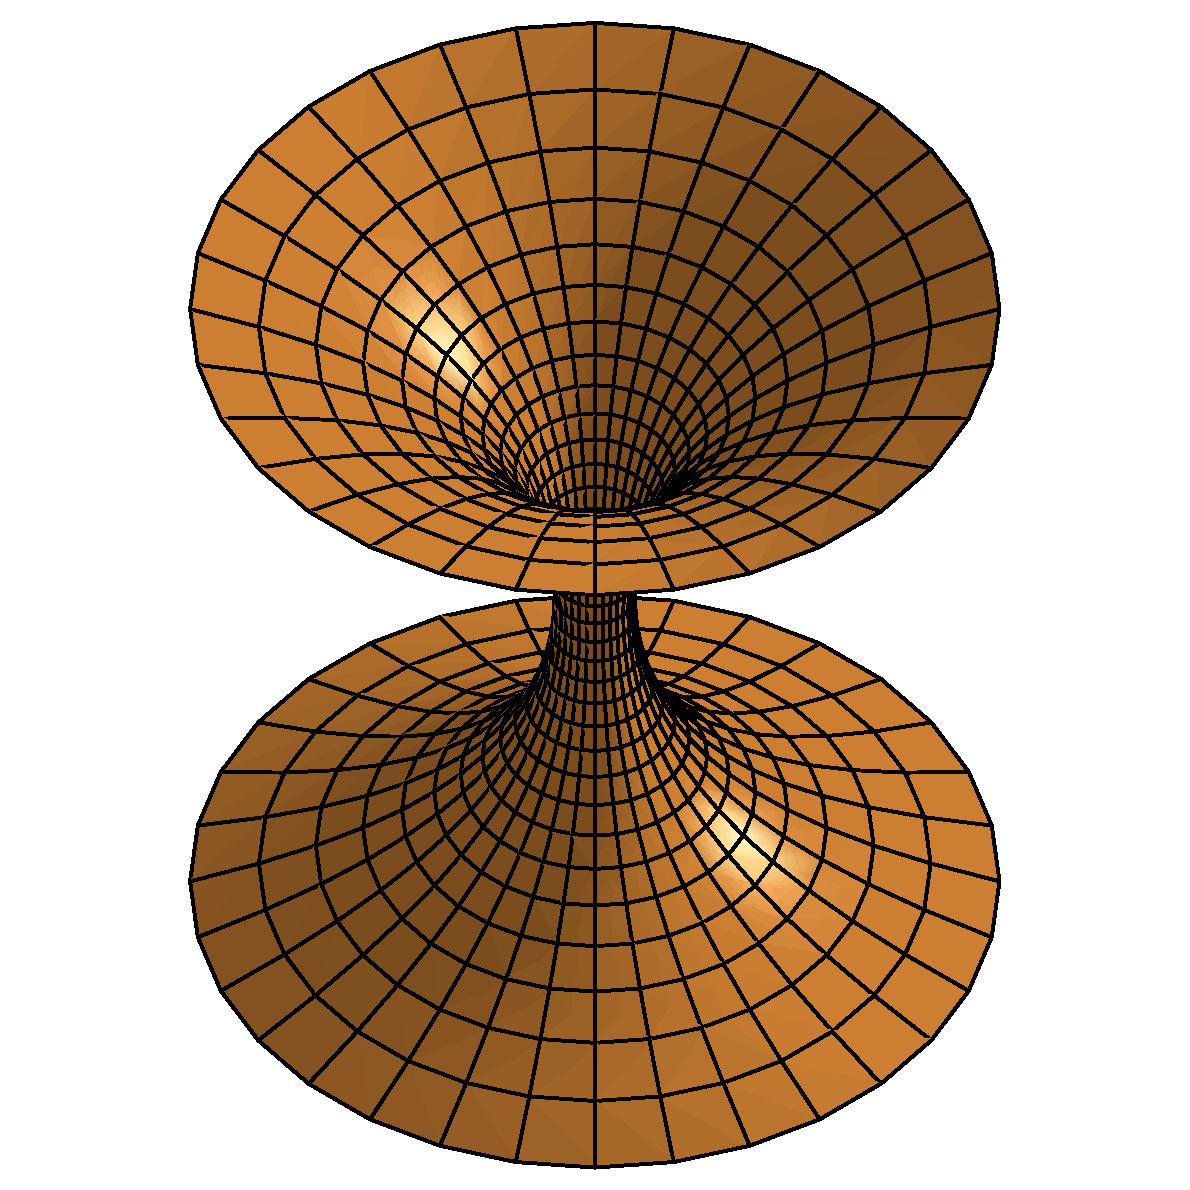
\includegraphics[width=8cm]{Images/Catenoid.eps}
   \caption{The Catenoid}
   \label{fig:catenoid}
\end{figure} 

\subsection{Ruled Surfaces}
We now apply another geometric constraint, asking that the surface be ruled.
\begin{definition}
A ruled surface is a surface parametrised by
\begin{displaymath}
\mathbf x(u,v) = \beta(u) + v \gamma(u)
\end{displaymath}

Such that we have straight lines starting on the curve $\beta(u)$ going in the direction $\gamma(u)$.
\end{definition}

There are many examples of ruled surfaces and the above definition becomes immediately obvious having seen a few.

\begin{example}[The Plane]
\begin{displaymath}
\mathbf x(u,v) =  \left[ \begin{array}{c} u\\0\\0 \end{array} \right] + v\left[ \begin{array}{c} 0\\1\\0 \end{array} \right] = \left[ \begin{array}{c} u\\v\\0 \end{array} \right]
\end{displaymath}

The plane in fact has two rulings as can be seen in figure \ref{fig:plane}. Also since it is flat it is also a minimal surface.

\begin{figure}[htbp]
	\centering
       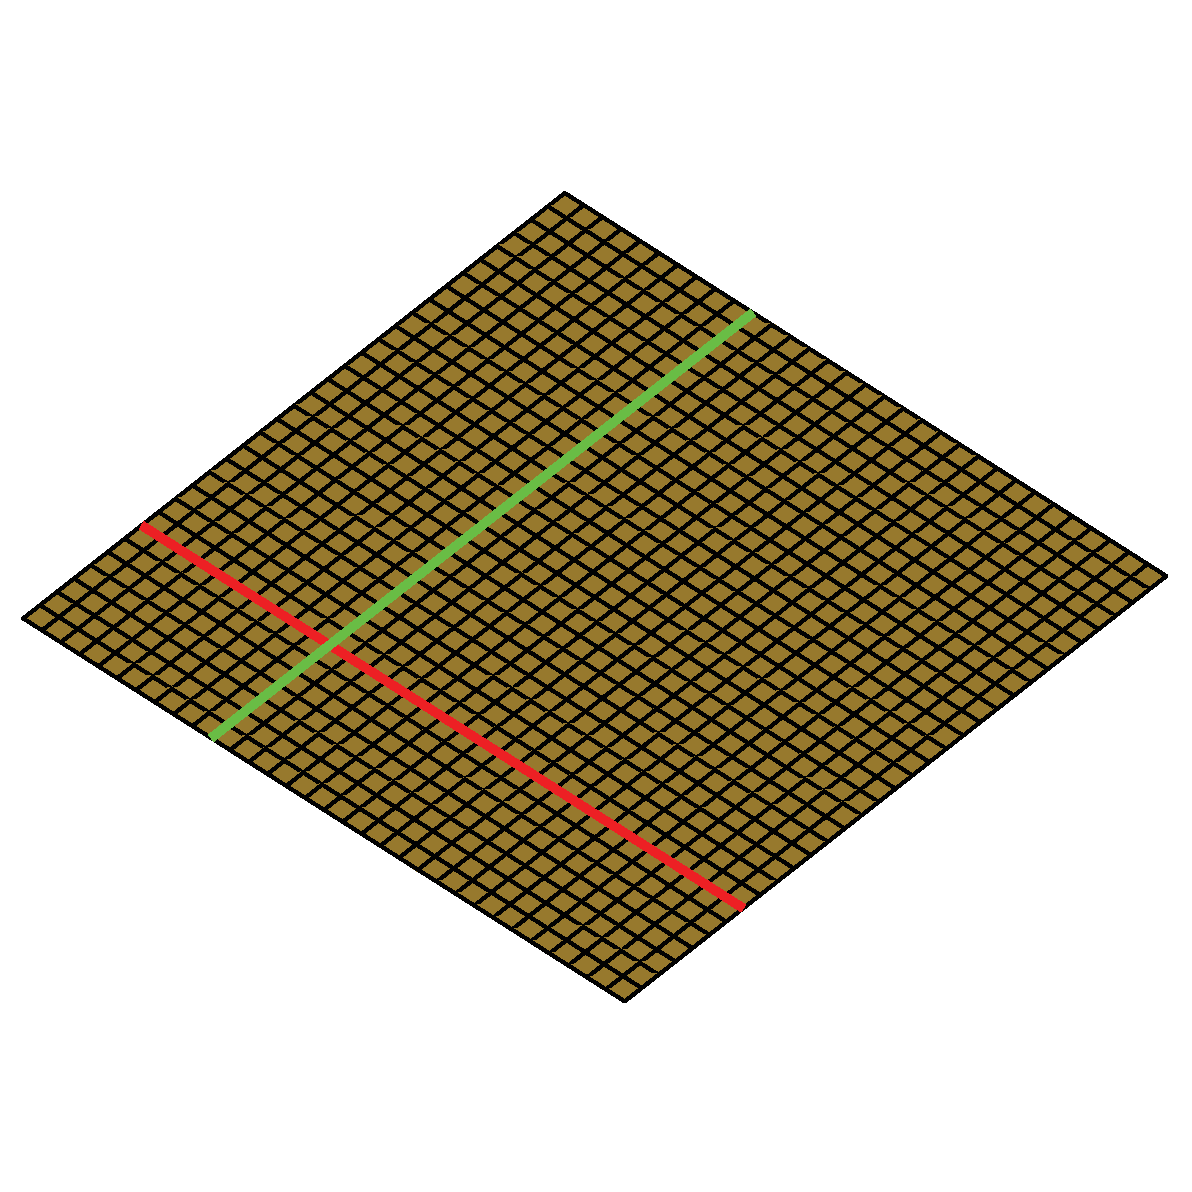
\includegraphics[width=8cm]{Images/Plane.eps}
   \caption{The Plane}
   \label{fig:plane}
\end{figure} 
\end{example}

\begin{example}[The Cone]
\begin{displaymath}
\mathbf x(u,v) =  \left[ \begin{array}{c} 0\\0\\0 \end{array} \right] + v\left[ \begin{array}{c} 1\\ \cos u \\ \sin u \end{array} \right] = \left[ \begin{array}{c} v\\v \cos u \\v \sin u \end{array} \right]
\end{displaymath}

See Figure \ref{fig:cone}.

\begin{figure}[htbp]
	\centering
       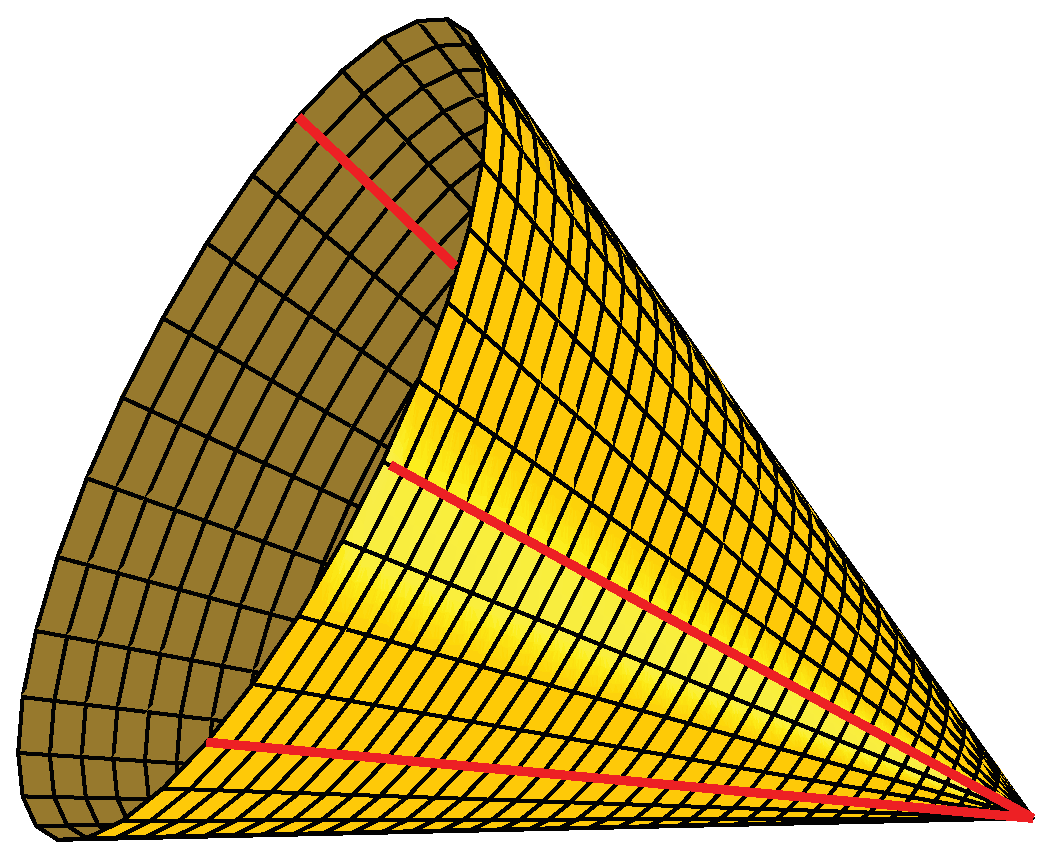
\includegraphics[width=8cm]{Images/Cone.eps}
   \caption{The Cone}
   \label{fig:cone}
\end{figure} 
\end{example}

\begin{example}[The Helicoid]
\begin{displaymath}
\mathbf x(u,v) = (a\:\sinh \: v\: cos \: u, a \: \sinh \:v \: \sin \:u, au)
\end{displaymath}

See Figure \ref{fig:helicoid}

\begin{figure}[htbp]
	\centering
       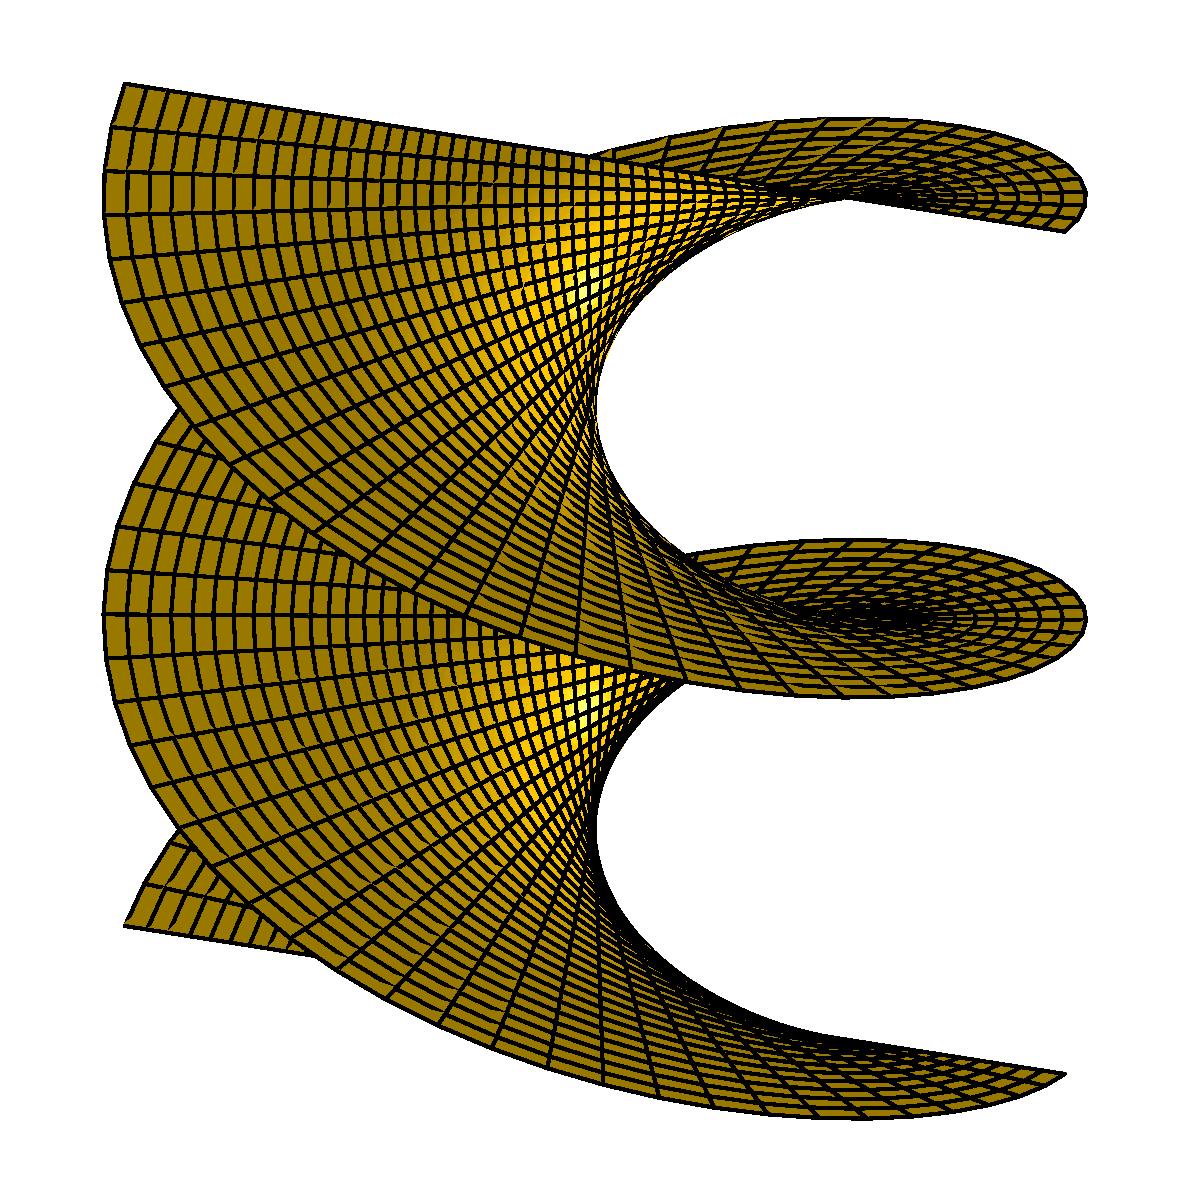
\includegraphics[width=8cm]{Images/Helicoid.eps}
   \caption{The Helicoid}
   \label{fig:helicoid}
\end{figure} 

Calculating as before $E=G= a^2cosh^2v$, $F = 0$, $L = M = 0$, $N = a^2$ gives $H=0$. So the Helicoid is a Minimal Surface.
\end{example}

\begin{theorem}
\label{Ruled}
The Helicoid is the only ruled minimal surface, other than the plane.
\label{RuledMinimal}
\end{theorem}
The proof of this requires the following:

\begin{lemma}
The zeros of the Gaussian curvature of a minimal surface are isolated.
\end{lemma}

\begin{definition}[Asymptotic Curve]
Let p be a point in S. An asymptotic direction of S at p is a direction of $T_p(S)$ for which the normal curvature is zero. An asymptotic curve of S is a regular connected curve $C \subset S$ such that for each $p \in C$ the tangent line of C at p is an asymptotic direction.
\end{definition}

\begin{definition}[Osculating Plane]
The plane determined by the unit tangent and normal vectors to a space curve as seen in figure \ref{fig:oscplane}.
\begin{figure}[htbp]
	\centering
       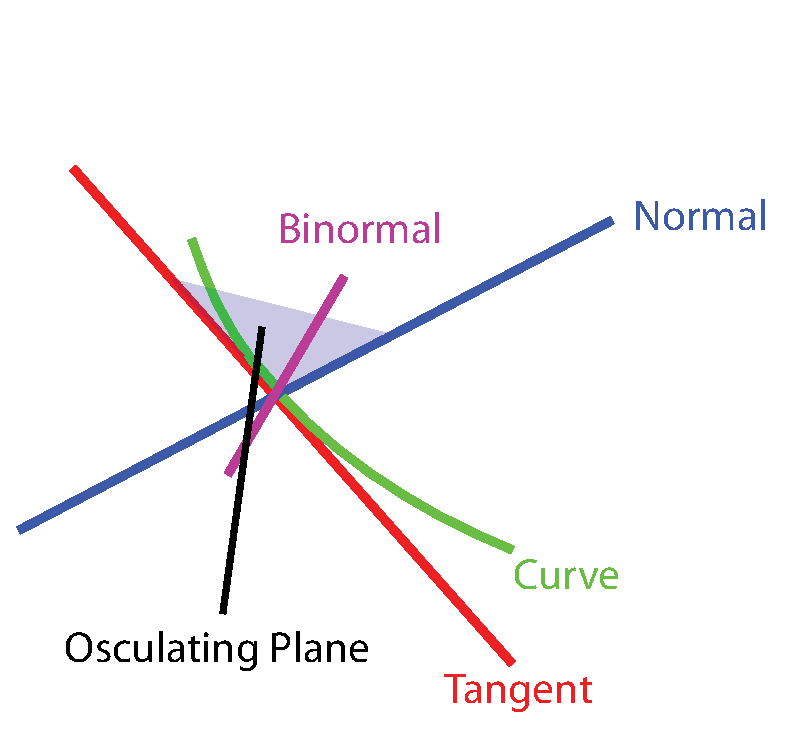
\includegraphics[width=8cm]{Images/OsculatingPlane.eps}
   \caption{Osculating Plane}
   \label{fig:oscplane}
\end{figure}
\end{definition}

\begin{definition}[Torsion]
This is the rate of change of the Osculating Plane as you move along the curve.
\end{definition}

\begin{definition}[Bertrand Curve]
let $\alpha: I \rightarrow R^3$ be a parametrised regular curve with $k(t) \neq 0$, $\tau \neq 0$, $t \in I$. The curve $\alpha$ is called a Bertrand curve if there exists a curve $\overline{\alpha}: I \rightarrow R^3$ such that the normal lines of $\alpha$ and $\overline{\alpha}$ at $t \in I$ are equal. In this case, $\overline{\alpha}$ is called a Bertrand mate of $\alpha$, and we can write

\begin{displaymath}
\overline{\alpha}= \alpha(t) + rn(t)
\end{displaymath}

\end{definition}

\begin{lemma}
If $\alpha$ has more than one Bertrand mate, it has infinitely many Bertrand mates. This case occurs if and only if $\alpha$ is a circular helix.
\label{lem:CircHelix}
\end{lemma}

\begin{proof}{Theorem \ref{RuledMinimal}}. 

Let S be a minimal ruled surface, $H=0$ and assume S is not a plane.

In some region W of S the Gaussian curvature K is strictly negative.

\begin{displaymath}
H =\frac{1}{2} (\kappa_1+\kappa_2) = 0 \Leftrightarrow \kappa_1 = -\kappa_2
\end{displaymath}

\begin{displaymath}
\Leftrightarrow K=\kappa_1 \cdot \kappa_2 < 0
\end{displaymath}

Given that S is minimal, $H=0$ and therefore W is covered by two families of asymptotic curves which intersect orthogonally. 

Since the rulings are asymptotic curves and the surface is not a plane, we can choose a point $q \in W$ such that the asymptotic curve, other than the ruling, passing though q has nonzero torsion at q.

Since the osculating plane of an asymptotic curve is the tangent plane to the surface, there exists a region in $W$ such that the rulings in this region are principal normals to the family of twisted asymptotic curves.

Lemma \ref{lem:CircHelix} says that this occurs if and only if the twisted curves are circular helices.

Therefore this region is a part of a Helicoid.

Since the torsion of a circular helix is constant, it can be seen that the whole surface is part of a Helicoid, as we claimed.
\end{proof}


